\chapter{Introdução}
\label{cap-introducao}

Pesquisas sobre Empreendedorismo são antigas, algumas datando meados do século XIX, e embora ainda não haja um consenso sobre qual a sua definição já sabemos que é uma disciplina que pode ser aprendida, as pessoas não nascem Empreendedoras mas são criadas para se tornarem Empreendedores. 

Também já sabemos bastante sobre as dinâmicas e quais as boas práticas de Empreendedores e Empresas de sucesso, mas pouco sabemos sobre Ecossistemas e como eles contribuem para o desenvolvimento das pessoas que os cercam. É notável que Ecossistemas tem uma grande influência no sucesso da Economia, das Empresas e das Pessoas do local, caso contrário não haveriam grandes centros Empreendedores como o Vale do Silício, Nova Iorque ou Tel-Aviv, mas mesmo com tantos exemplos famosos no mundo inteiro pouco se sabe sobre como seus diversos elementos interagem entre si para que tenhamos um Ecossistema Vibrante. Alguns pesquisadores como \citeonline{Suresh2012} já tentaram mapear elementos que são essenciais para o sucesso de um Ecossistema.

\citeonline{Cukier2016} relata que o interesse pelo tema é crescente nos últimos anos, representado por meio da Figura XX com o aumento da quantidade de artigos acadêmicos que referenciem o termo ``Startup Ecosystem''.

\begin{figure}[!htb]
\centering
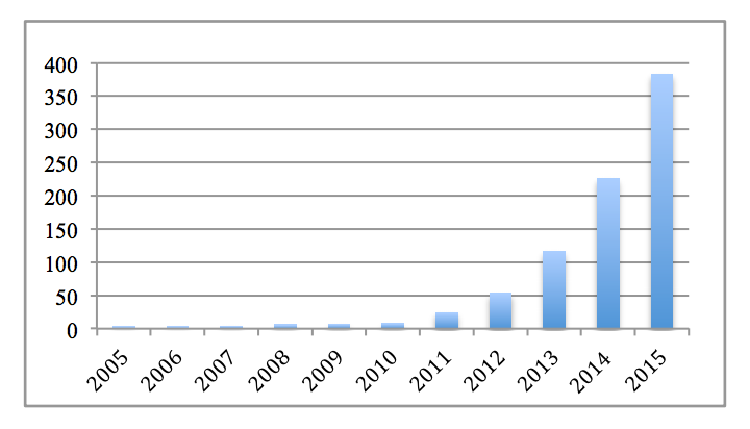
\includegraphics[width=11cm,angle=0]{figuras/papers_about_startup_ecosystems}
\caption{Quantidade de Papers com o termo ``Startup Ecosystem'' por \citeonline{Cukier2016}}
\label{figure:papers_about_startup_ecosystems}
\end{figure}

\citeonline{Lemos2011} diz que pesquisas sobre ecossistemas de empreendedorismo apresentam um forte caráter exploratório e que faltam teorias consolidadas sobre as relações entre os diversos elementos que compõem um Ecossistema. Infelizmente, esse trabalho não será diferente, mas a expectativa é que ele represente tanto o começo da vida acadêmica de um pesquisador com a temática de Ecossistemas como também represente o começo de uma série de pesquisas sobre as Startups de Brasília. 

\citeonline{Paternoster2014} enfatiza que pesquisas acadêmicas são necessárias para apoiar as atividades das Startups para ajuda-los a tomar decisões e evitar escolher que poderiam resultar em falhas.

Em uma entrevista para o site da Revista Times\footciteref{Phillips2014} a Empreendedora brasileira Bel Pesce relata que em apenas duas semanas após o lançamento do seu primeiro livro na internet ele obteve mais de cem mil downloads, o que a motivou a abrir a escola de empreendedorismo FazInova\footciteref{fazinova} que no primeiro ano obteve cerca de nove mil estudantes. Hoje a plataforma possui mais de 150 mil usuários e o conteúdo criado pela Empreendedora já atingiu mais de 5 milhões de pessoas nos últimos 3 anos por meio de revistas, programas de televisão ou rádio, palestras, YouTube, etc. Ela relata que as pessoas nem sequer piscam durante as atividades, que os brasileiros querem empreender.

Brasília, em especial, é a casa de diversos casos de sucesso no contexto de Startups do Brasil. Em entrevista ao Correio Braziliense\footciteref{menezes2012} Júlio Vasconcellos, ex-morador de Brasília e um dos fundadores do Peixe Urbano, acredita que a capital possui um excelente sistema de educação e jovens com talento e ambição e que o contexto político da cidade, que atrai muitos estrangeiros e brasileiros de todas as regiões do país, contribui para a geração de um ambiente dinâmico e favorável para o desenvolvimento de jovens empreendedores. 

A Boo-Box, uma das maiores empresas de publicidade digital do mundo e adquirida pela FTPI Digital, a ZeroPaper, adquirida pela americana Intuit, a Rota dos Concursos, a primeira Startup brasileira a participar do programa de aceleração 500 Startups no Vale do Silício, também são grandes nomes da capital. Em 2016, a Tradr, criada em Brasília, recebeu o prêmio de melhor Startup na área de e-commerce na Campus Party Brasil.

\section{Contexto}
\label{section:contexto}

Atualmente Brasília vive um dos seus melhores momentos para as Startups, embora o país esteja passando uma recessão e no meio de uma crise política e econômica o cenário nunca foi tão favorável, o Ecossistema está se se movimentando. 

Atualmente é possível encontrar eventos com temáticas empreendedoras toda semana, como palestras e meetups. Em 2016 e 2017 Brasília também receberá edições do maior evento de tecnologia, inovação e empreendedorismo do mundo: a Campus Party. A baixa expectativa de concursos públicos também é um fator favorável, forçando os jovens a considerarem novas alterantivas que não a estabilidade financeira incentivada pelos seus pais e principal motivo para uma Cultura Empreendedora tão ruim.

Em relação a financiamento existem dois fundos de alto risco com aproximadamente R\$ 100 milhões para investimento em Startups, o Criatec 2, sob resposabilidade da Garan Ventures, e o Fundo de Investimento em Participações Venture Brasil Central, sob responsabilidade da Cedro Capital. Também temos três programas de aceleração de Startups rodando na cidade, o Programa Impulso, o CAMP da aceleradora Cotidiano, e a Acceleratus. 

Em relação ao governo local, a Fundação de Apoio à Pesquisa em 2015 e 2016 investiu cerca de R\$ 13 milhões em Startups locais. Em relação ao governo federal, as Startups de Brasília tem acesso à iniciativas como o Startup Brasil, Inovativa Brasil, Sebrae de Inovacão (R\$20 milhões para o programa e até R\$ 120 por projeto) e Editais da FINEP.

A presença de cerca de dez espaços de coworking, incluindo um totalmente gratuito, também atuam como importantes atores para o desenvolvimento do Ecossistema.

\section{Objetivos}
\label{section:objetivos}

Tenho como missão realizar um estudo exploratório do Ecossistema de Startups do Distrito Federal com o objetivo de conhece-lo. 

Ao fim deste trabalho espera-se que seja obtido como resultado uma visão geral de como os principais fatores que compõem esse Ecossistema interagem entre si por meio da criação de um [Mapa Conceitual], bem como algumas de suas características e ações que poderiam ser tomadas para que Brasília se tornasse mais forte e unida.

De cunho pessoal, tenho como objetivo utilizar este trabalho como pretexto para me integrar ao Ecossistema, aumentar minha rede de contatos, aprender com pessoas mais experientes e ajudar conforme eu consiga. De cunho profissional, espero visualizar problemas e soluções que eu possa trazer para que seja solucionado no contexto Governamental, onde atuo na área de Fomento ao Empreendedorismo.

\section{Organização do Trabalho}
\label{section:organizacao_do_trabalho}

Este trabalho está organizado em cinco capítulos: o primeiro, este, com uma breve introdução de suas motivações, objetivos e contexto. 

O segundo capítulo, com foco na Fundamentação Teórica trás diversos conceitos e visões relativos ao Empreendedorismo, sobre quem é o Empreendedor e o que é uma Startup, bem como o seu Ciclo de Vida e o seu mercado fora do convencional. 

O terceiro capítulo explora a Metodologia utilizada, como as entrevistas foram realizadas, como esse trabalho se relaciona com outros similares, etc. 

O quarto capítulo trás os Resultados Obtidos, o que foi descoberto, qual a visão dos Empreendedores entrevistados, etc.

No último capítulo, o de Conclusões, é feito um apanhado de tudo o que foi explorado nos capítulos anteriores e o que fora aprendido sobre o Ecossistema de Startups do Distrito Federal e quais ações poderiam ser tomadas para que Brasília se torne uma cidade mais empreendedora.